\documentclass[12pt,letterpaper]{article}
\usepackage{fullpage}
\usepackage[top=2cm, bottom=4.5cm, left=2.5cm, right=2.5cm]{geometry}
\usepackage{amsmath,amsthm,amsfonts,amssymb,amscd}
\usepackage{lastpage}
\usepackage{enumerate}
\usepackage{fancyhdr}
\usepackage{mathrsfs}
\usepackage{xcolor}
\usepackage{graphicx}
\usepackage{listings}
\usepackage{hyperref}
\usepackage{tikz}
\usepackage{xfrac}
\usepackage{nicefrac}
\usepackage{xcolor}

\usetikzlibrary{shapes.geometric,fit}

\hypersetup{
    colorlinks=true,
    linkcolor=blue,
    linkbordercolor={0 0 1}
}

\setlength{\parindent}{0.0in}
\setlength{\parskip}{0.05in}

\newcommand\course{ECON 3211}
\newcommand\hwnumber{6}
\newcommand\NetIDa{dc3451}
\newcommand\NetIDb{David Chen}

\theoremstyle{definition}
\newtheorem*{statement}{Statement}
\newtheorem*{claim}{Claim}
\newtheorem*{theorem}{Theorem}

\newcommand{\contra}{\Rightarrow\!\Leftarrow}
\newcommand{\Lag}{\mathcal{L}}

\pagestyle{fancyplain}
\headheight 35pt
\lhead{\NetIDa}
\lhead{\NetIDa\\\NetIDb}
\chead{\textbf{\Large Problem Set \hwnumber}}
\rhead{\course \\ \today}
\lfoot{}
\cfoot{}
\rfoot{\small\thepage}
\headsep 1.5em

\begin{document}

\section*{Problem 1}

\subsection*{a)}

We have that $q(\lambda L,\lambda K) = (\lambda L)^{0.5}(\lambda K)^{0.5} =
\lambda L^{0.5}K^{0.5} = \lambda q(L,K)$, so we have constant returns to scale.

\subsection*{b)}

In India, we have that $\frac{MP_L}{MP_K} = \frac{w}{r} = 1 \implies
\frac{0.5L^{-0.5}K^{0.5}}{0.5L^{0.5}K^{-0.5}} = \frac{K}{L} = 1$, so we have that
the firm hires one unit of labor for each unit of capital.

\subsection*{c)}

The lowest cost while producing 100 units of output in India is $q(L^*,K^*) =
q(L^*,L^*) = L^* = 100 \implies L^* = K^* = 100$. The total cost is then $wL + rK =
8(100) + 8(100)=  \$1600$.

\subsection*{d)}

In Mexico, we have that $\frac{MP_L}{MP_K} = \frac{K}{L} = \frac{w}{r} = 4
\implies 4L = K$. Thus, for each unit of labor, the firm purchases four units of capital.

\subsection*{e)}

The lowest cost while producing 100 units of output in Mexico is $q(L^*,K^*) =
q(L^*,4L^*) = 2L^* = 100 \implies L^* = 50, K^* = 200$. The total cost is then
$wL + rK = 50(16) + 200(4) = \$1600$.

\subsection*{f), g)}

\begin{center}
  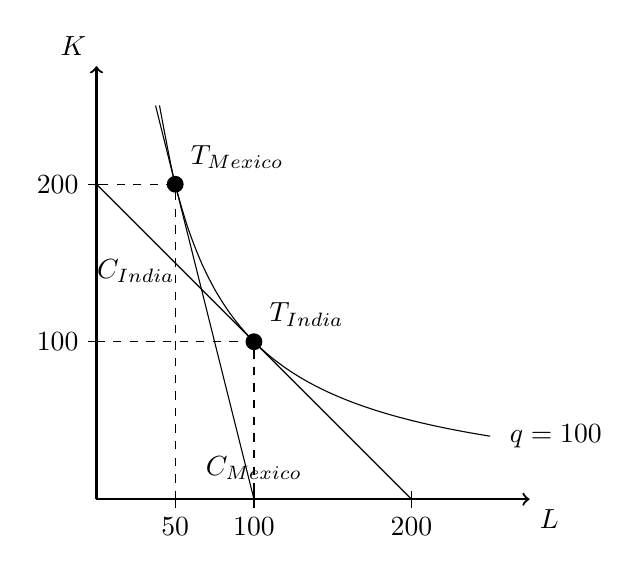
\begin{tikzpicture}[
    dot/.style={shape=circle, inner sep=2pt, draw, node contents=},
    circ/.style={shape=circle, inner sep=2pt, draw, fill}]
    \draw[thick,->] (0,0) -- (5.5,0) node[anchor=north west] {$L$};
    \draw[thick,->] (0,0) -- (0,5.5) node[anchor=south east] {$K$};

    \draw[domain=40:250,scale=0.02,smooth,variable=\x] plot ({\x},{10000/\x}) node[label=right:{$q = 100$}]{};
    \draw (2cm,3pt) -- (2cm,-3pt) node[anchor=north] {$100$}; 
    \draw (4cm,3pt) -- (4cm,-3pt) node[anchor=north] {$200$}; 
    \draw (1cm,3pt) -- (1cm,-3pt) node[anchor=north] {$50$}; 
    \draw (3pt,2cm) -- (-3pt,2cm) node[anchor=east] {$100$};
    \draw (3pt,4cm) -- (-3pt,4cm) node[anchor=east] {$200$};

    \draw (0,4) -- node[label={$C_{India}$},xshift=-15mm,yshift=5mm]{} (4,0);
    \draw (0.75,5) -- (2,0) node[label=above:{$C_{Mexico}$}]{};

    \draw (2,2) node[circ,label=above right:{$T_{India}$}]{};
    \draw (1,4) node[circ,label=above right:{$T_{Mexico}$}]{};
    \draw[dashed] (0,2) -- (2,2) -- (2,0);
    \draw[dashed] (1,0) -- (1,4) -- (0,4);
  \end{tikzpicture}
\end{center}

\subsection*{h)}

The company does not relocate to Mexico, as the total cost of the minimizing
techniques are still the same at $\$1600$.

\subsection*{i)}

No, the firm's decision is not dependent on the target output level, as we have
that $L^*_{India} = K^*_{India} = q, L^*_{Mexico} = \frac{1}{2}q,
K^*_{Mexico} = 2q \implies C_{India} = C_{Mexico} = 16q$.

\subsection*{j)}

\subsubsection*{j.1}

\[
  \min_{L,K} wL + rK \text{ s.t. } L^{0.5}K^{0.5} = q
\]

\subsubsection*{j.2}

\begin{align*}
  \Lag(L,K,\lambda) &= wL + rK - \lambda (L^{0.5}K^{0.5} - q) \\
  \frac{\partial \Lag}{\partial L} &= w - 0.5\lambda L^{-0.5}K^{0.5} = 0 \\
  \frac{\partial \Lag}{\partial K} &= r - 0.5\lambda L^{0.5}K^{-0.5} = 0 \\
  \frac{\partial \Lag}{\partial \lambda} &= -L^{0.5}K^{0.5} + q = 0 \\
\end{align*}

\subsubsection*{j.3}

\begin{alignat*}{2}
  && \frac{w}{r} &= \frac{K}{L} \\
  &\implies& K &= \frac{wL}{r} \\
  &\implies& (\frac{w}{r})^{0.5}L &= q \\
  &\implies& \hat{L} &= (\frac{r}{w})^{0.5}q \\
  && L &= \frac{rK}{w} \\
  &\implies& (\frac{r}{w})^{0.5} K &= q \\
  &\implies& \hat{K} &= (\frac{w}{r})^{0.5}q
\end{alignat*}

If the firm wishes to double production, it doubles the amount of workers as
well as the amount of capital.

\subsubsection*{j.4}

\begin{align*}
  C &= w\hat{L} + r\hat{K} \\
    &= \sqrt{rw}q + \sqrt{rw}q \\
    &= 2\sqrt{rw}q
\end{align*}

\subsubsection*{j.5}

\[
  AC = \frac{C}{q} = 2\sqrt{rw}
\]

The average cost is constant.

\section*{Problem 2}

\subsection*{a)}

% Technology exhibits decreasing returns to scale: $q(L,\lambda K) =
% 4\lambda^{\frac{1}{3}}L^{\frac{1}{3}}K^{\frac{1}{3}} < 4\lambda
% L^{\frac{1}{3}}K^{\frac{1}{3}} = \lambda q(L,K)$.

In general, the firm exhibits decreasing returns to scale: $q(\lambda L, \lambda
K) = 4\lambda^{\frac{2}{3}}L^{\frac{1}{3}}K^{\frac{1}{3}} < 4\lambda
L^{\frac{1}{3}}K^{\frac{1}{3}} = \lambda q(L,K)$.

\subsection*{b)}

Because we have that the production function is Cobb-Douglas, the firm spends
$\frac{\frac{1}{3}}{\frac{1}{3} + \frac{1}{3}} = \frac{1}{2}$ of the total
expenditure on labor and also $\frac{\frac{1}{3}}{\frac{1}{3} + \frac{1}{3}} =
\frac{1}{2}$ of the total expenditure on equipment. This share does not depend
on $q$.

\subsection*{c)}

The average cost ought to be increasing, as we have decreasing returns to scale,
which then transfers over to average cost in that the firm operates in
diseconomies of scale.

\section*{Problem 3}

\subsection*{a)}

Since she uses 10 apples, 10 sticks, and 20 oz of sugar, the total cost is going
to be $10(1) + 10(0.5) + 0.2(5) = 10 + 5 + 1 = \$16$. This assumes that she can
divide the purchases evenly; for example, if she cannot divide the purchase of
sugar, then she will need to spend $10 + 5 + 5 = \$20$, with 80 oz sugar left over.

\subsection*{b)}
There is only one reasonable technique here, as the inputs are perfect
complements to each other. Specifically, in order to make $q$ candied apples, Sarah is
going to use $q$ apples, $q$ sticks, $2q$ oz of sugar, for a total cost
$C(q,P_A,P_{WS},P_S) = qP_a + qP_{WS} + 2qP_S$.

\section*{Problem 4 (Joe)}

\subsection*{a)}
Joe's variable cost is going to be, if he optimizes, be entirely incurred by
spending on the more efficient California oranges, as we have that $\frac{MP_C}{P_C} = 0.5 >
\frac{MP_F}{P_F} = 0.4$. Thus, since he needs $C = \frac{q}{0.5} = 2q$
California oranges to produce $q$, he has to spend $C(q) = 2q$ as the variable cost.

\subsection*{b)}

\begin{center}
  \begin{tikzpicture}[
    dot/.style={shape=circle, inner sep=2pt, draw, node contents=},
    circ/.style={shape=circle, inner sep=2pt, draw, fill}]
    \draw[thick,->] (0,0) -- (5.5,0) node[anchor=north west] {$C$};
    \draw[thick,->] (0,0) -- (0,5.5) node[anchor=south east] {$F$};

    \draw (4cm,3pt) -- (4cm,-3pt) node[anchor=north] {$2\bar{q}$}; 
    \draw (3pt,5cm) -- (-3pt,5cm) node[anchor=east] {$2.5\bar{q}$};

    \draw (0,5) -- node[label=right:{$q = \bar{q}$}]{} (4,0);
    \draw (0,4) -- node[label=left:{$C = 2\bar{q}$}]{} (4,0);
    \draw (4,0) node[circ,label=above right:{$T$}]{};
  \end{tikzpicture}
\end{center}

\section*{Problem 4 (Mr. X)}

\subsection*{a)}

\[
  \Pi(L) = 9(10\sqrt{L}) - 3(10\sqrt{L}) - 15L = 60\sqrt{L} - 15L
\]

\subsection*{b)}

To maximize profit, we want $\frac{d\Pi}{dL} = 30L^{-0.5} - 15 = 0 \implies
L^{0.5} = 2 \implies L = 4$.

\subsection*{c)}

Mr. X pays $3(10\sqrt{L}) = 30(2) = \$ 60$ every day, making $60(2)- 15(4) = \$
60$ in profit.

\subsection*{d)}

His new profit function is then

\[
  \Pi(L) = 90\sqrt{L} - 15L - 70
\]

The first order condition is then $\frac{d\Pi}{dL} = 45L^{-0.5} - 15 = 0 \implies
L = 9$, up from $4$.

\subsection*{e)}

Mr. X now makes $\Pi(L) = 90\sqrt{9} - 15(9) - 70 = \$65$ in profit. It is
unclear whether Mr. X should take the new arrangement, as we no idea how he
prefers his leisure time (he may actually value it greater than minimum wage,
meaning that in some of these cases he would keep the old arrangement).

% If, for example, he simply cares about taking the
% situation in which he makes higher hourly profit, he should take the old deal,
% as he makes $60 / 4 = \$15 / hr$ , and the new deal makes $65 / 9 = \$7.22 / hr$
% in profit.

On the other hand, if he values other time exactly at minimum wage, then he should
actually switch!

\section*{Problem 5}
\subsection*{a)}

Low productivity:

\begin{align*}
  \Pi_L(L) &= pq - wL - FC = 2L^{0.5} - wL \\
  \frac{d\Pi_L}{dL} &= L^{-0.5} - w = 0 \\
  L &= w^{-2}
\end{align*}

High productivity:

\begin{align*}
  \Pi_H(L) &= pq - wL - FC = 4L^{0.5} - wL \\
  \frac{d\Pi_L}{dL} &= 2L^{-0.5} - w = 0 \\
  L &= 4w^{-2}
\end{align*}

\subsection*{b)}

Computing, $AD = \sum L = 10(w^{-2}) + 10(4w^{-2}) = 50w^{-2}$.

\subsection*{c)}

We want that $AD = AS$ in the labor market, so $50w^{-2} = 200 \implies w =
0.5$, and $L_L = 4, L_H = 16$.

\subsection*{d)}

\begin{center}
  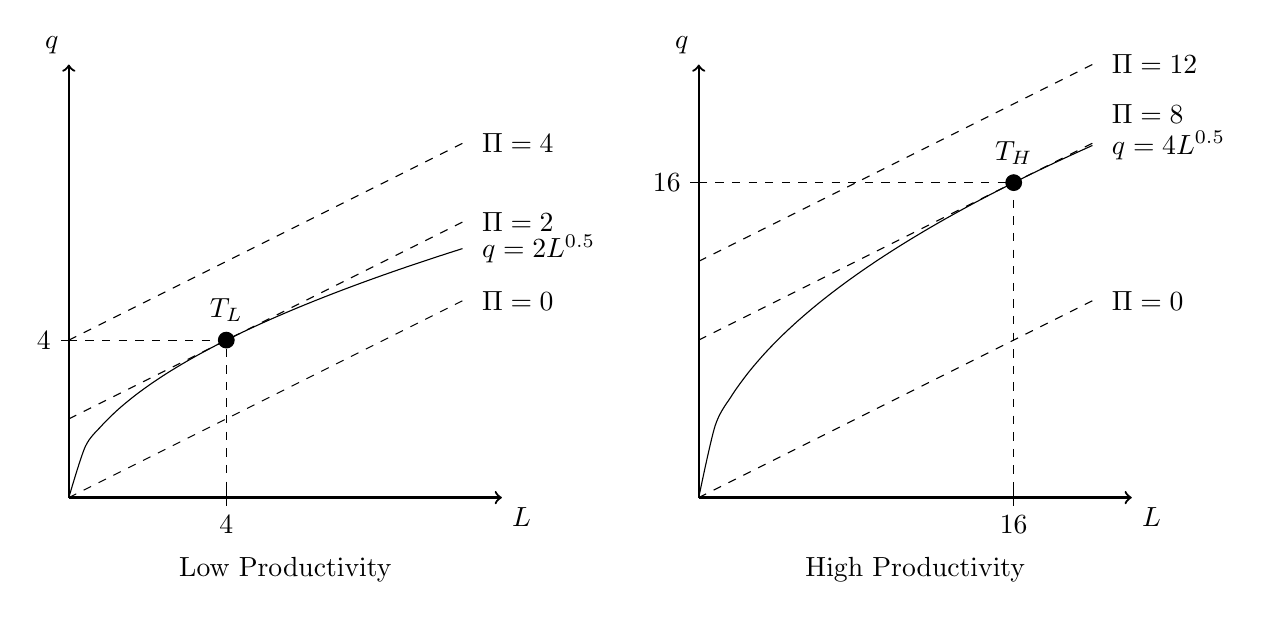
\begin{tikzpicture}[
    dot/.style={shape=circle, inner sep=2pt, draw, node contents=},
    circ/.style={shape=circle, inner sep=2pt, draw, fill}]
    \draw[thick,->] (0,0) -- node[label=below:{Low Productivity},yshift=-5mm]{}(5.5,0) node[anchor=north west] {$L$};
    \draw[thick,->] (0,0) -- (0,5.5) node[anchor=south east] {$q$};

    \draw[thick,->] (8,0) -- node[label=below:{High Productivity},yshift=-5mm]{} (13.5,0) node[anchor=north west] {$L$};
    \draw[thick,->] (8,0) -- (8,5.5) node[anchor=south east] {$q$};

    \draw[domain=0:10,scale=0.5,smooth,variable=\x] plot ({\x},{2*sqrt(\x)}) node[label=right:{$q = 2L^{0.5}$}]{};
    \draw[domain=0:20,scale=0.25,smooth,variable=\x] plot ({\x+32},{4*sqrt(\x)}) node[label=right:{$q = 4L^{0.5}$}]{};

    \draw[dashed] (0,0) -- (5,2.5) node[label=right:{$\Pi = 0$}]{};
    \draw[dashed] (0,1) -- (5,3.5) node[label=right:{$\Pi = 2$}]{};
    \draw[dashed] (0,2) -- (5,4.5) node[label=right:{$\Pi = 4$}]{};

    \draw[dashed] (8,0) -- (13,2.5) node[label=right:{$\Pi = 0$}]{};
    \draw[dashed] (8,2) -- (13,4.5) node[label=above right:{$\Pi = 8$}]{};
    \draw[dashed] (8,3) -- (13,5.5) node[label=right:{$\Pi = 12$}]{};

    \draw[dashed] (0,2) -- (2,2) -- (2,0);
    \draw[dashed] (8,4) -- (12,4) -- (12,0);

    \draw (2,2) node[circ,label=above:{$T_L$}]{};
    \draw (12,4) node[circ,label=above:{$T_H$}]{};

    \draw (2cm,3pt) -- (2cm,-3pt) node[anchor=north] {$4$}; 
    \draw (12cm,3pt) -- (12cm,-3pt) node[anchor=north] {$16$}; 
    \draw (3pt,2cm) -- (-3pt,2cm) node[anchor=east] {$4$};
    \draw (8cm+3pt,4cm) -- (8cm-3pt,4cm) node[anchor=east] {$16$};
  \end{tikzpicture}
\end{center}

\subsection*{e)}

\begin{alignat*}{2}
  && \min_{L_L,L_H} 10(2L_L^{0.5}) + 10(4L_H^{0.5}) &\text{ s.t. } 10L_L + 10L_H = 200\\
  && \Lag(L_L,L_H,\lambda) &= 20L_L^{0.5} + 40L_H^{0.5} - \lambda(10L_L + 10L_H - 200)
  \\
  && \frac{\partial \Lag}{\partial L_L} &= 10L_L^{-0.5} - \lambda = 0 \\
  && \frac{\partial \Lag}{\partial L_H} &= 20L_H^{-0.5} - \lambda = 0 \\
  && \frac{\partial \Lag}{\partial \lambda} &= -10L_L - 10L_H + 200 = 0 \\
  &\implies& 2L^{-0.5}_H &= L_L^{-0.5} \\
  &\implies& L_H &= 4L_L \\
  &\implies& 50L_L = 200 \\
  &\implies& L_L&= 4 \\
  &\implies& L_H &= 16
\end{alignat*}

To guarantee efficiency.

\subsection*{f)}

The market demand for labor contributed from the low productivity firms is
unchanged. However, in the high productivity firms, we now see that
\begin{align*}
  \Pi(L) &= 4L^{0.5} - 1.5wL \\
  \frac{d\Pi}{dL} &= 2L^{-0.5} - 1.5w = 0 \\
  L^{-0.5} &= \frac{3w}{4} \\
  L &= \frac{16}{9}w^{-2}
\end{align*}

Computing $AD = \sum L = 10(w^{-2}) + 10(\frac{16}{9}w^{-2}) = \frac{250}{9}w^{-2}$.

\subsection*{g)}

The labor supply is still inelastic at 200, so we have that $\frac{250}{9}w^{-2}
= 200 \implies w = \frac{\sqrt{5}}{6} = 0.37$. The wage has gone down (which
makes sense, since demand has also shrunk).

\subsection*{h)}

After, we have that $L_L = w^{-2} = \frac{36}{5} > 4, L_H = \frac{16}{9}w^{-2} =
\frac{64}{5} < 16$. Thus, labor has shifted toward the lower production firms.

\subsection*{i)}

As for allocation, we have that before the tax, total production was
$10(2(4^{-0.5})) + 10(4(16^{-0.5})) = 40 + 160 = 200$.

After the tax, total production is $10(2(\frac{36}{5})^{-0.5}) +
10(4(\frac{64}{5})^{-0.5}) = \frac{120}{\sqrt{5}} + \frac{320}{\sqrt{5}} =
\frac{440}{\sqrt{5}} = 88\sqrt{5} = 196.8$. Total production has decreased, so
efficiency is not fully achieved in allocation.

\subsection*{j)}

Labor would return to full efficiency. The workers would eat the entire impact
of the tax in their wages, so labor allocation returns to $L_L= 4, L_H = 16$. We
can be formally seen in that in low productivity firms, $\Pi(L) = 2L^{0.5} -
1.5wL \implies \frac{d\Pi}{dL} = L^{-0.5} - 1.5w = 0 \implies L =
\frac{4}{9}w^{-2}$, and in high productivity firms, $\Pi(L) = 4L^{0.5} - 1.5wL
\implies L = \frac{16}{9}w^{-2}$. Total demand for labor is then
$10(\frac{4}{9})w^{-2} + 10(\frac{16}{9})w^{-2} = \frac{200}{9}w^{-2}$. Setting
this equal to supply, $\frac{200}{9}w^{-2} = 200 \implies w = \frac{1}{3}$.
Then, $L_L = \frac{4}{9}w^{-2} = 4, L_H = \frac{16}{9}w^{-2} = 16$, and labor is
again efficiently allocated.

\end{document}